\title{Assignment 3: CS 736, Algorithms for Medical Image Processing}
\author{Alankar Kotwal -- 12D070010, Riddhish Bhalodia -- 120070003}

\documentclass[11pt]{article}

\usepackage{amsmath}
\usepackage{amssymb}
\usepackage{hyperref}
\usepackage{ulem}
\usepackage{graphicx}
\usepackage{float}
\usepackage[margin=0.5in]{geometry}

\begin{document}
\maketitle
\section*{Part (a)}

\begin{figure}[H]
\caption{IFFT of K-space Data}
\centerline{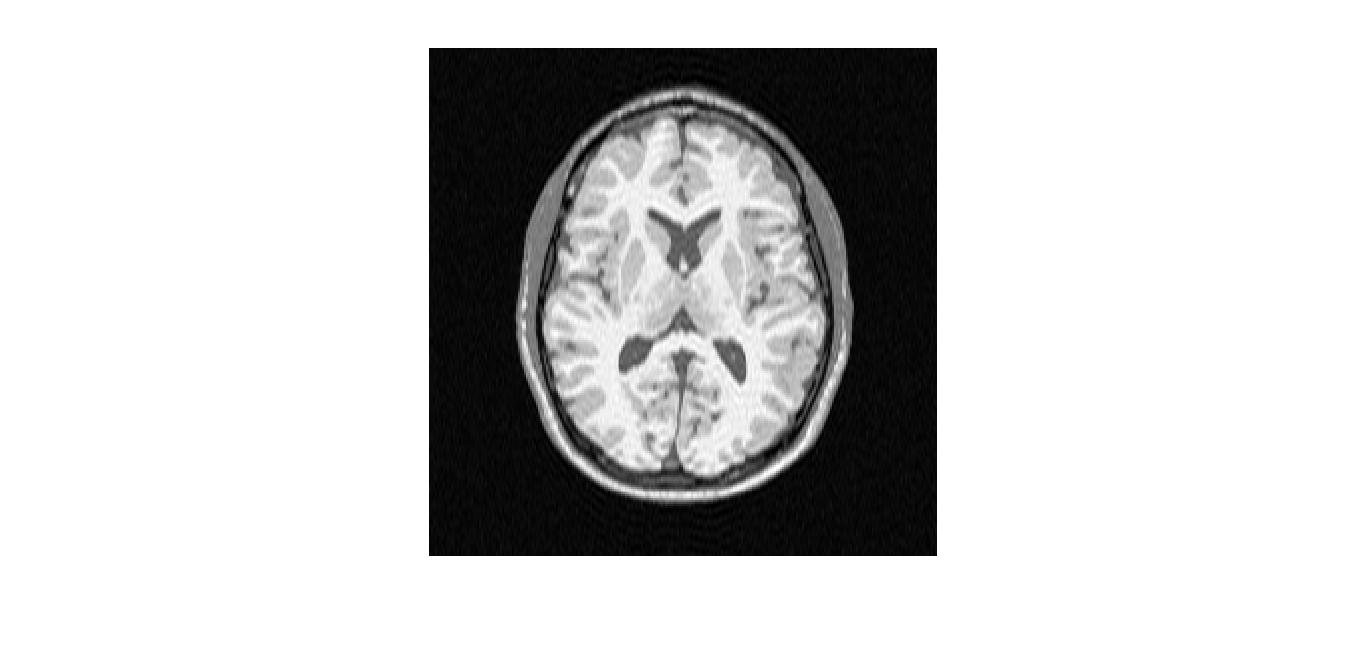
\includegraphics[scale=0.3]{ifft}}
\end{figure}

\begin{figure}[H]
\caption{Image reconstructed with Quadratic prior}
\centerline{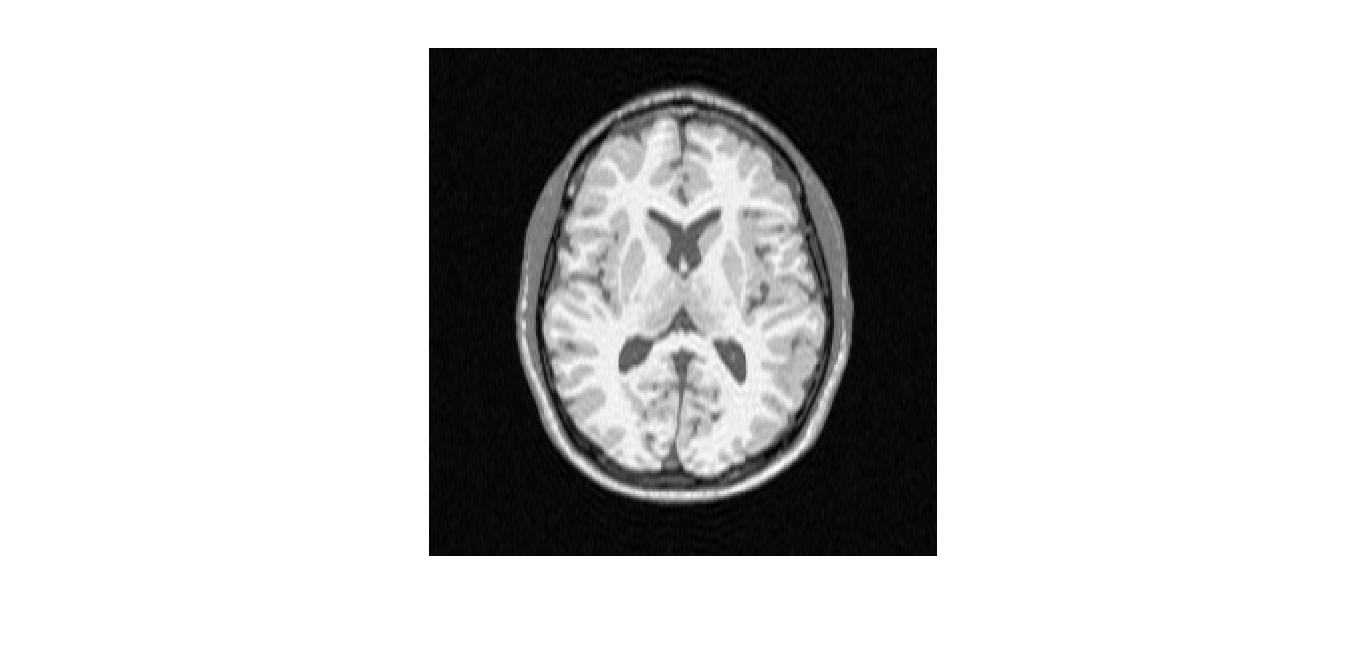
\includegraphics[scale=0.3]{quadRec}}
\end{figure}

\begin{figure}[H]
\caption{Image reconstructed with Huber prior}
\centerline{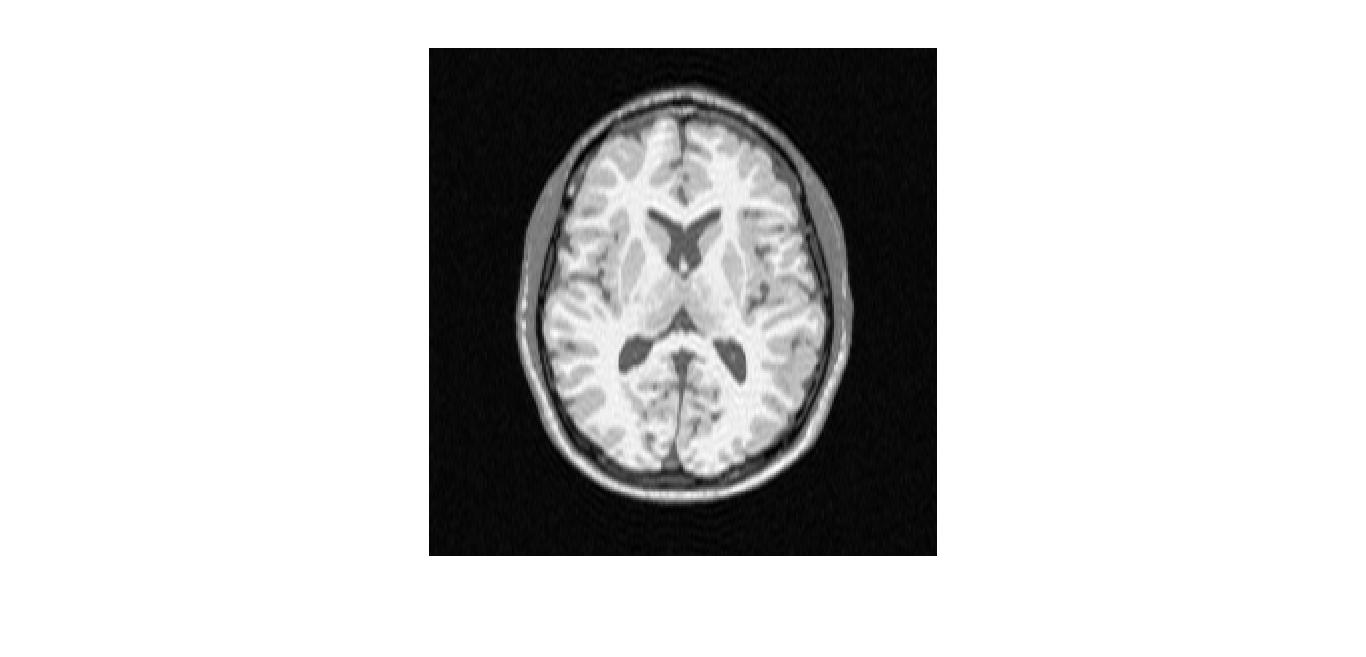
\includegraphics[scale=0.3]{huberRec}}
\end{figure}

\begin{figure}[H]
\caption{Image reconstructed with Discontinuity-adaptive prior}
\centerline{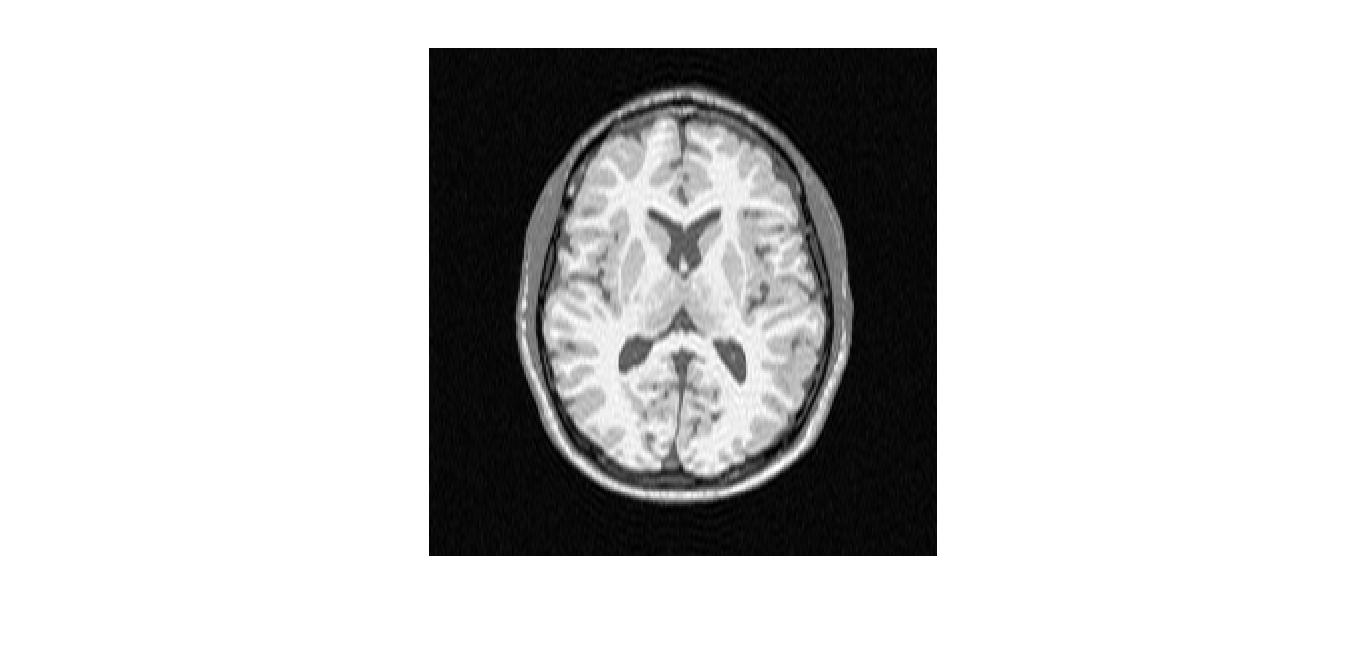
\includegraphics[scale=0.3]{discRec}}
\end{figure}

\section*{Part (b)}

\begin{figure}[H]
\caption{Quadratic prior objective function}
\centerline{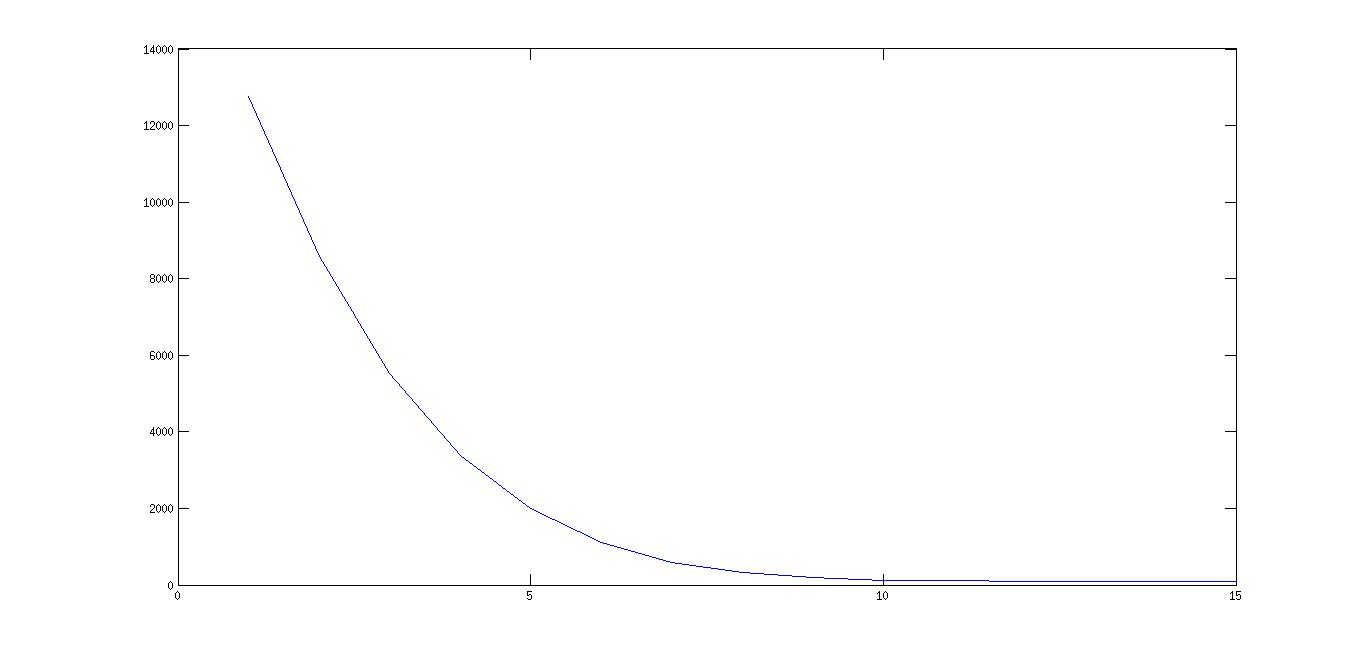
\includegraphics[scale=0.3]{quadObj}}
\end{figure}

\begin{figure}[H]
\caption{Huber prior objective function}
\centerline{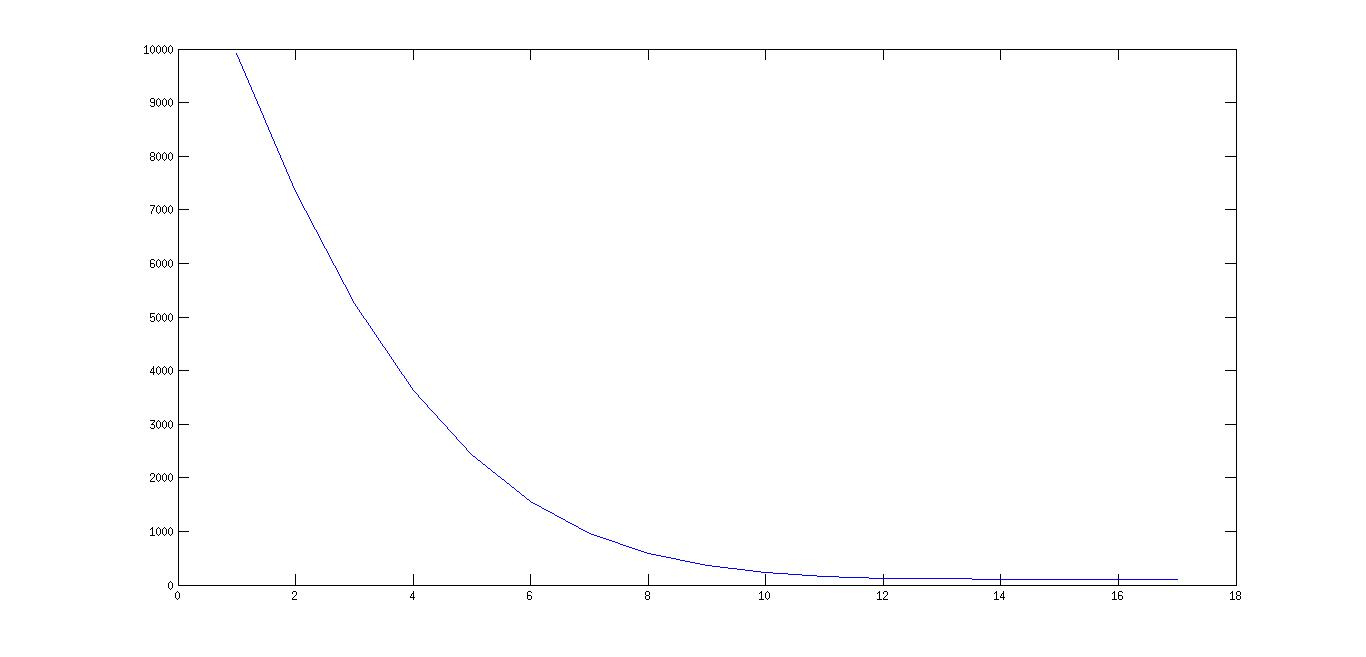
\includegraphics[scale=0.3]{huberObj}}
\end{figure}

\begin{figure}[H]
\caption{Discontinuity-adaptive prior objective function}
\centerline{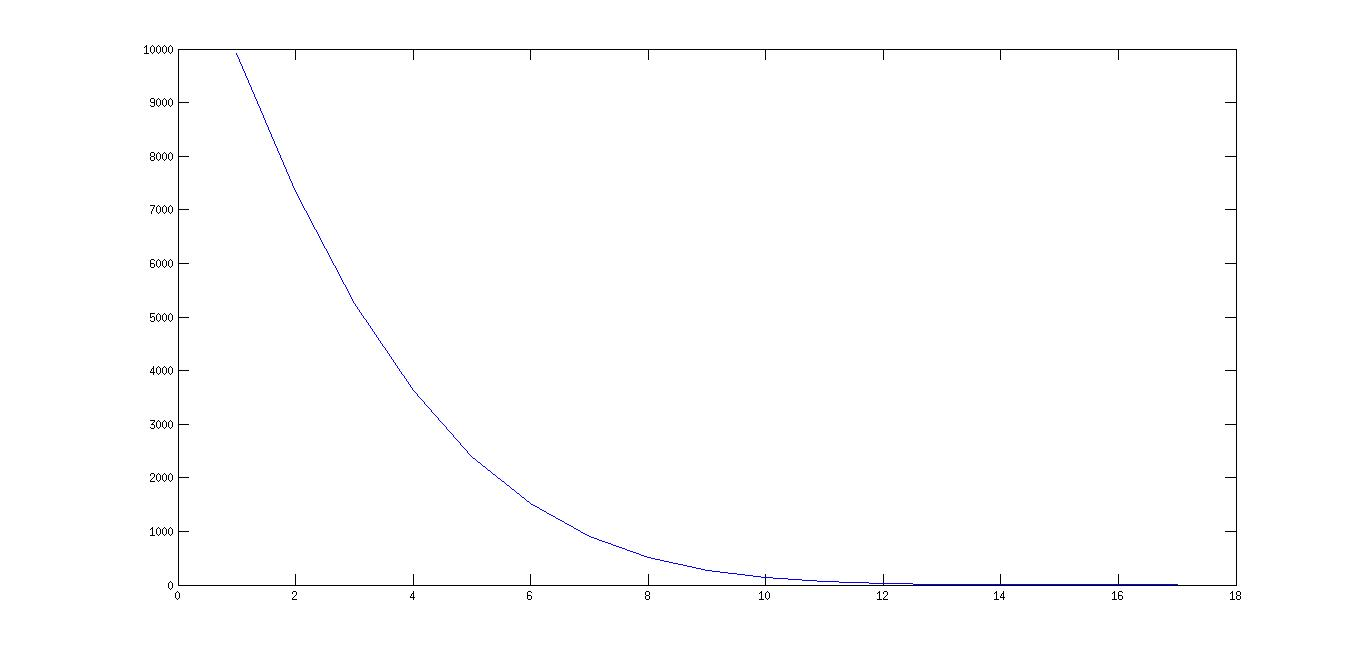
\includegraphics[scale=0.3]{discObj}}
\end{figure}

\end{document}